%%%% This is based on the Beamer example was created by LianTze Lim, April 2017.

\documentclass[14pt]{beamer}

%%%%%%%%%%%%%%%%%%%%%%%%%%%%%%%%%%%%%%%%%%%%%%%%%%%%%%%%%%%%%%%%%%%%%%%%%%%%%%%%

    \usepackage[english]{babel}
    \usepackage[utf8]{inputenc}
    \usepackage[T1]{fontenc}
    \usepackage{lmodern}
    \usepackage{textcomp}
    \usepackage[cm]{sfmath}
    \usepackage[euler]{textgreek}

    \usepackage{xfrac}

    %% Set the left and right margins
    \setbeamersize{text margin left=1em,text margin right=1em}

    %% Fonts
    \setbeamerfont{title}{series=\bfseries,size=\huge}
    \setbeamerfont{subtitle}{series=\bfseries,size=\large}
    \setbeamerfont{date}{size=\footnotesize}
    \setbeamerfont{frametitle}{series=\bfseries,size=\large}
    \setbeamerfont{block title}{series=\bfseries,size=\large}
    \setbeamerfont{footline}{size=\normalsize}

    %% Colors
    \setbeamercolor{background canvas}{bg=white!5!black}    % Blackboard
    \setbeamercolor{structure}{fg=white!95!black}           % Chalk
    \usebeamercolor{structure}
    \setbeamercolor{normal text}{fg=structure.fg}

    %% Add a line after the frametitle
    \setbeamertemplate{frametitle}[default][left,leftskip=1ex]
    \addtobeamertemplate{frametitle}{}{\vspace*{-1ex}\rule{\textwidth}{2pt}}

    %% Use circular discs as itemized list markers
    \setbeamertemplate{itemize items}[circle]

    %% Remove default navigation symbols
    \setbeamertemplate{navigation symbols}{}

    %% Remove the footline
    \setbeamertemplate{footline}{}

%%%%%%%%%%%%%%%%%%%%%%%%%%%%%%%%%%%%%%%%%%%%%%%%%%%%%%%%%%%%%%%%%%%%%%%%%%%%%%%%

\title{The Egyptian Tangram}
\subtitle{Properties of a new 5-piece tangram\vspace{-1.0em}}
\author{
    
\includegraphics[height=15ex]{figures/figure001a.pdf}\\
    \vspace{0.75em}
    {\small \textcopyright\ \href{https://github.com/CarlosLunaMota}{Carlos Luna-Mota}}\\
    \vspace{0.75em}
    \href{https://mmaca.cat/}{
\includegraphics[width=10ex]{figures/logo.png}}\\
    \vspace{-1.75em}}
\date{\today}

\begin{document}

    %%%%%%%%%%%%%%%%%%%%%%%%%%%%%%%%%%%%%%%%%%%%%%%%%%%%%%%%%%%%%%%%%%%%%%%%%%%%

    \begin{frame}
      \titlepage
    \end{frame}

    %%%%%%%%%%%%%%%%%%%%%%%%%%%%%%%%%%%%%%%%%%%%%%%%%%%%%%%%%%%%%%%%%%%%%%%%%%%%

    \begin{frame}{}
        \begin{center}
            \textbf{\huge The Egyptian Tangram}
        \end{center}
    \end{frame}

    %%%%%%%%%%%%%%%%%%%%%%%%%%%%%%%%%%%%%%%%%%%%%%%%%%%%%%%%%%%%%%%%%%%%%%%%%%%%

    \begin{frame}{The Egyptian Tangram}
        \begin{center}
            
\includegraphics[height=20ex]{figures/figure001a.pdf} \\

            \bigskip

            A square dissection firstly proposed as a tangram in:

            \bigskip

            {\footnotesize Luna-Mota, C. (2019) \emph{``El tangram egipci: diari de disseny''} Nou Biaix, 44}
        \end{center}
    \end{frame}

    %%%%%%%%%%%%%%%%%%%%%%%%%%%%%%%%%%%%%%%%%%%%%%%%%%%%%%%%%%%%%%%%%%%%%%%%%%%%

    \begin{frame}{Origins}
        \begin{center}
            The Egyptian Tangram inspiration comes from\\the study of two other 5-piece tangrams...

            \bigskip

            
\includegraphics[height=18ex]{figures/figure000a.pdf} \qquad 
\includegraphics[height=18ex]{figures/figure000b.pdf} \\

            \bigskip

            {\small The ``Five Triangles'' \& ``Greek-Cross'' tangrams}
        \end{center}
    \end{frame}

    %%%%%%%%%%%%%%%%%%%%%%%%%%%%%%%%%%%%%%%%%%%%%%%%%%%%%%%%%%%%%%%%%%%%%%%%%%%%

    \begin{frame}{Origins}
        \begin{center}
            ...and their underlying grids\\\phantom{the study of two other 5-piece tangrams...}

            \bigskip

            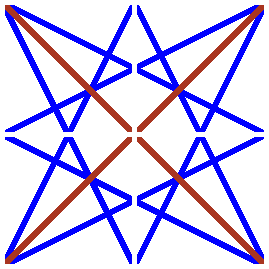
\includegraphics[height=18ex]{figures/figure000d.pdf} \qquad 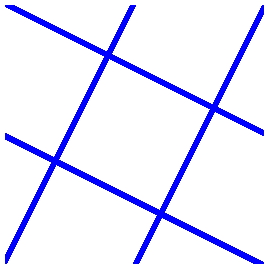
\includegraphics[height=18ex]{figures/figure000c.pdf} \\

            \bigskip

            {\small The ``Five Triangles'' \& ``Greek-Cross'' underlying grids}
        \end{center}
    \end{frame}

    %%%%%%%%%%%%%%%%%%%%%%%%%%%%%%%%%%%%%%%%%%%%%%%%%%%%%%%%%%%%%%%%%%%%%%%%%%%%

    \begin{frame}{Design Process}
        \begin{center}
            The Egyptian Tangram was the result of\\an heuristic incremental design process:

            \bigskip

            {\small Take a square and keep adding ``the most interesting straight cut'' until you have a dissection with 5 or more pieces.}

            \bigskip \bigskip


            
\includegraphics[height=10ex]{figures/figure001e.pdf} \quad 
\includegraphics[height=10ex]{figures/figure001d.pdf} \quad 
\includegraphics[height=10ex]{figures/figure001c.pdf} \quad 
\includegraphics[height=10ex]{figures/figure001b.pdf} \\
        \end{center}
    \end{frame}

    %%%%%%%%%%%%%%%%%%%%%%%%%%%%%%%%%%%%%%%%%%%%%%%%%%%%%%%%%%%%%%%%%%%%%%%%%%%%

    \begin{frame}{Design Process}
        \begin{center}
            
\includegraphics[height=18ex]{figures/figure001b.pdf}
        \end{center}

        To make an Egyptian Tangram:

        {\small \begin{enumerate}
            \item Connect the midpoint of the lower side with the upper corners.
            \item Connect the midpoint of the left side with the top right corner.
        \end{enumerate}}
    \end{frame}

    %%%%%%%%%%%%%%%%%%%%%%%%%%%%%%%%%%%%%%%%%%%%%%%%%%%%%%%%%%%%%%%%%%%%%%%%%%%%

    \begin{frame}{Antecedents}
        \begin{center}
            It turns out that this figure is not new...

            \bigskip \bigskip \bigskip

            {\small See problem 3 from:}

            \medskip

            {\footnotesize Detemple, D. \& Harold, S. (1996) \emph{``A Round-Up of Square Problems''} Mathematics Magazine, 69:1}

            \bigskip \bigskip \bigskip

            ...but, to the best of our knowledge,\\nobody used it before \textbf{as a tangram}
        \end{center}
    \end{frame}

    %%%%%%%%%%%%%%%%%%%%%%%%%%%%%%%%%%%%%%%%%%%%%%%%%%%%%%%%%%%%%%%%%%%%%%%%%%%%

    \begin{frame}{Antecedents}
        \begin{center}
            The name is not new either...

            \bigskip \bigskip

            
\includegraphics[height=15ex]{figures/figure000e.pdf}

            \medskip

            {\footnotesize This dissection is often called ``Egyptian Puzzle'' or ``Egyptian Tangram''}

            \bigskip \bigskip

            ...but there is a good reason to consider\\ our dissection the real ``Egyptian Tangram''\\{\footnotesize (even if it was designed in Barcelona)}
        \end{center}
    \end{frame}

    %%%%%%%%%%%%%%%%%%%%%%%%%%%%%%%%%%%%%%%%%%%%%%%%%%%%%%%%%%%%%%%%%%%%%%%%%%%%

    \begin{frame}{Antecedents}
        \begin{center}
            The underlying grid is also a well known figure:

            \bigskip \bigskip

            
\includegraphics[height=15ex]{figures/figure002b.pdf}\\

            \bigskip

            {\footnotesize Brunés, T. (1967) \emph{``The Secrets of Ancient Geometry -- and Its Use''}}

            \medskip

            {\footnotesize Bankoff, L. \& W. Trigg, C. (1974) \emph{``The Ubiquitous 3:4:5 Triangle''}, Mathematics Magazine, 47:2}
        \end{center}
    \end{frame}

    %%%%%%%%%%%%%%%%%%%%%%%%%%%%%%%%%%%%%%%%%%%%%%%%%%%%%%%%%%%%%%%%%%%%%%%%%%%%

    \begin{frame}{The pieces}
        \begin{center}

            \begin{minipage}{17.5ex}\vspace{2ex}
                
\includegraphics[height=17ex]{figures/figure001a.pdf}\\
            \end{minipage}\begin{minipage}{30ex}
                \footnotesize
                \begin{itemize}
                    \item Just five pieces
                    \item All pieces are different
                    \item All pieces are asymmetric
                    \item Areas are integer and not \emph{too different}
                    \item All sides are multiples of $1$ or $\sqrt{5}$
                    \item All angles are linear combinations of $90^\circ$ and \textalpha\ $= \arctan{\!\left(\tfrac{1}{2}\right)} \approx 26,565^\circ$
                \end{itemize}
            \end{minipage}

            \smallskip

            {\footnotesize
            \begin{tabular}{c|c|l|l}
                \;\;\textbf{Name}\;\; & \;\;\textbf{Area}\;\; & \;\;\textbf{Sides}          & \;\;\textbf{Angles} \\ \hline
                \textbf{T1}   & $1$           & \;\;$1,\; 2,\; \sqrt{5}$          & \;\;$90,\; \text{\textalpha},\; 90\!-\!\text{\textalpha}$   \\ \hline
                \textbf{T4}   & $4$           & \;\;$2,\; 4,\; 2\sqrt{5}$         & \;\;$90,\; \text{\textalpha},\; 90\!-\!\text{\textalpha}$   \\ \hline
                \textbf{T5}   & $5$           & \;\;$\sqrt{5},\; 2\sqrt{5},\; 5$  & \;\;$90,\; \text{\textalpha},\; 90\!-\!\text{\textalpha}$   \\ \hline
                \textbf{T6}   & $6$           & \;\;$3,\; 4,\; 5$                 & \;\;$90,\; 90\!-\!2\text{\textalpha},\; 2\text{\textalpha}$ \\ \hline
                \textbf{Q4}   & $4$           & \;\;$1,\; 3,\; \sqrt{5},\; \sqrt{5}$\;\; & \;\;$90,\; 90\!-\!\text{\textalpha},\; 90,\; 90\!+\!\text{\textalpha}$\;\;
            \end{tabular}}
        \end{center}
    \end{frame}

    %%%%%%%%%%%%%%%%%%%%%%%%%%%%%%%%%%%%%%%%%%%%%%%%%%%%%%%%%%%%%%%%%%%%%%%%%%%%

    \begin{frame}{The pieces}
        \begin{center}
            Although all pieces are asymmetric and different,\\they often combine to make symmetric shapes

            \bigskip \bigskip

            
\includegraphics[height=7ex]{figures/figure020a.pdf}\quad
\includegraphics[height=7ex]{figures/figure020b.pdf}\quad
\includegraphics[height=7ex]{figures/figure020c.pdf}\qquad
            
\includegraphics[height=7ex]{figures/figure020h.pdf}\quad
\includegraphics[height=7ex]{figures/figure020i.pdf} \\ \bigskip
            
\includegraphics[height=7ex]{figures/figure020d.pdf}\quad
\includegraphics[height=7ex]{figures/figure020f.pdf} \quad 
\includegraphics[height=7ex]{figures/figure020e.pdf}\quad
\includegraphics[height=7ex]{figures/figure020g.pdf} \\ \bigskip
            
\includegraphics[height=3ex]{figures/figure020k.pdf}\quad
\includegraphics[height=3ex]{figures/figure020j.pdf} \\ \medskip
            
\includegraphics[height=3ex]{figures/figure020m.pdf}\quad
\includegraphics[height=3ex]{figures/figure020l.pdf} \\
        \end{center}
    \end{frame}

    %%%%%%%%%%%%%%%%%%%%%%%%%%%%%%%%%%%%%%%%%%%%%%%%%%%%%%%%%%%%%%%%%%%%%%%%%%%%

    \begin{frame}{The pieces}
        \begin{center}
            This means that it is very rare for an Egyptian Tangram figure to have a unique solution

            \bigskip \bigskip

            
\includegraphics[height=12ex]{figures/figure021a.pdf}\quad
\includegraphics[height=12ex]{figures/figure021b.pdf}\quad
\includegraphics[height=12ex]{figures/figure021c.pdf} \\

            \vspace{2em}

            {\footnotesize There are three different solutions for the square and, in all three cases,\\two of the corners of the square are built as a sum of acute angles!}
        \end{center}
    \end{frame}

    %%%%%%%%%%%%%%%%%%%%%%%%%%%%%%%%%%%%%%%%%%%%%%%%%%%%%%%%%%%%%%%%%%%%%%%%%%%%

        \begin{frame}{Why we called it the \emph{Egyptian} Tangram?}
        \begin{center}
            The smallest pieces of the Xinese and Greek-Cross Tangrams can be used to build all the other pieces...

            \bigskip \bigskip

            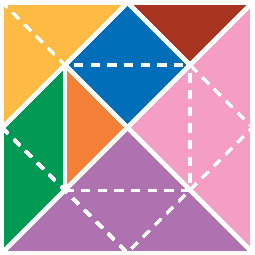
\includegraphics[height=15ex]{figures/figure003c.pdf}\quad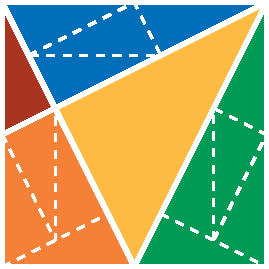
\includegraphics[height=15ex]{figures/figure003a.pdf}\quad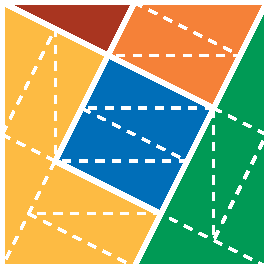
\includegraphics[height=15ex]{figures/figure003b.pdf} \\

            \bigskip \bigskip

            ...but you cannot do the same with\\the Egyptian Tangram because of T6
        \end{center}
    \end{frame}

    %%%%%%%%%%%%%%%%%%%%%%%%%%%%%%%%%%%%%%%%%%%%%%%%%%%%%%%%%%%%%%%%%%%%%%%%%%%%

    \begin{frame}{Why we called it the \emph{Egyptian} Tangram?}
        \begin{center}
            {\small Initially, T6 was considered as the \emph{leftover} piece that results from cutting all these $1\!\!:\!\!2\!\!:\!\!\sqrt{5}$ triangles from the borders of the square. But it turned out to be a very well known triangle...}

            \bigskip \bigskip

            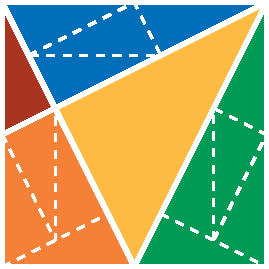
\includegraphics[height=15ex]{figures/figure003a.pdf} \\

            \bigskip \bigskip

            ...the \textbf{Egyptian} Triangle ($3\!\!:\!\!4\!\!:\!\!5$)\\{\small and, hence, the name}
        \end{center}
    \end{frame}

    %%%%%%%%%%%%%%%%%%%%%%%%%%%%%%%%%%%%%%%%%%%%%%%%%%%%%%%%%%%%%%%%%%%%%%%%%%%%

    \begin{frame}{}
        \begin{center}
            \textbf{\Huge Egyptian Tangram\\\bigskip Puzzles}\\
        \end{center}
    \end{frame}

    %%%%%%%%%%%%%%%%%%%%%%%%%%%%%%%%%%%%%%%%%%%%%%%%%%%%%%%%%%%%%%%%%%%%%%%%%%%%

    \begin{frame}{Geometric figures with all 5 pieces}

        \vspace{-1em}
        \begin{center}
            \begin{tabular}{lccc}
                    \raisebox{0.0ex}{
\includegraphics[scale=0.2]{figures/figure022a.pdf}} \;\;&
                \;\;\raisebox{0.0ex}{\rotatebox{90}{
\includegraphics[scale=0.2]{figures/figure022r.pdf}}} \;\;&
                \;\;\raisebox{0.0ex}{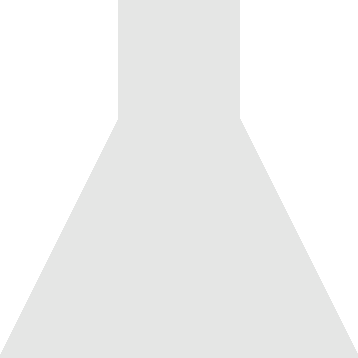
\includegraphics[scale=0.2]{figures/figure022u.pdf}} \;\;&
                \;\;\raisebox{0.0ex}{
\includegraphics[scale=0.2]{figures/figure022l.pdf}} \\[1.0ex]
                    \raisebox{1.0ex}{
\includegraphics[scale=0.2]{figures/figure022b.pdf}} \;\;&
                \;\;\raisebox{0.8ex}{
\includegraphics[scale=0.2]{figures/figure022j.pdf}} \;\;&
                \;\;\raisebox{0.8ex}{
\includegraphics[scale=0.2]{figures/figure022i.pdf}} \;\;&
                \;\;\raisebox{0.0ex}{
\includegraphics[scale=0.2]{figures/figure022p.pdf}} \\[0.750ex]
                    \raisebox{0.0ex}{
\includegraphics[scale=0.2]{figures/figure022e.pdf}} \;\;&
                \;\;\raisebox{0.0ex}{
\includegraphics[scale=0.2]{figures/figure022m.pdf}} \;\;&
                \;\;\raisebox{0.0ex}{
\includegraphics[scale=0.2]{figures/figure022h.pdf}} \;\;&
                \;\;\raisebox{0.0ex}{
\includegraphics[scale=0.2]{figures/figure022t.pdf}} \\[1.5ex]
                    \raisebox{0.0ex}{
\includegraphics[scale=0.2]{figures/figure022c.pdf}} \;\;&
                \;\;\raisebox{0.0ex}{
\includegraphics[scale=0.2]{figures/figure022n.pdf}} \;\;&
                \;\;\raisebox{0.0ex}{
\includegraphics[scale=0.2]{figures/figure022g.pdf}} \;\;&
                \;\;\raisebox{0.0ex}{\includegraphics[scale=0.2]{figures/figure022q.pdf}} \\[1.5ex]
                    \raisebox{0.0ex}{\includegraphics[scale=0.2]{figures/figure022d.pdf}} \;\;&
                \;\;\raisebox{0.0ex}{\includegraphics[scale=0.2]{figures/figure022o.pdf}} \;\;&
                \;\;\raisebox{0.0ex}{\includegraphics[scale=0.2]{figures/figure022k.pdf}} \;\;&
                \;\;\raisebox{0.0ex}{\includegraphics[scale=0.2]{figures/figure022s.pdf}} \\
            \end{tabular}
        \end{center}
    \end{frame}

    %%%%%%%%%%%%%%%%%%%%%%%%%%%%%%%%%%%%%%%%%%%%%%%%%%%%%%%%%%%%%%%%%%%%%%%%%%%%

    \begin{frame}{Realistic figures with all 5 pieces}
        \begin{center}
            {\footnotesize
            \begin{tabular}{ccc}
                \includegraphics[scale=0.3]{figures/figure026a.pdf} &
                \includegraphics[scale=0.3]{figures/figure026b.pdf} &
                \includegraphics[scale=0.3]{figures/figure026c.pdf}\\
                \;\;Viking hat & Snowmobile & Sailboat\\[1ex]
            \end{tabular}}

            \bigskip\bigskip

            We are looking for additional realistic figures!

            \bigskip\bigskip

            Please send yours to: \href{mailto:carlos.luna@mmaca.cat}{carlos.luna@mmaca.cat}
        \end{center}
    \end{frame}

    %%%%%%%%%%%%%%%%%%%%%%%%%%%%%%%%%%%%%%%%%%%%%%%%%%%%%%%%%%%%%%%%%%%%%%%%%%%%

    \begin{frame}{Sum of similar figures}
        \begin{center}
            Use all 5 pieces to build the single figure in the LHS,
            then use them to build the two figures on the RHS

            \bigskip\bigskip

            {\Huge \begin{tabular}{ccccc}
                \includegraphics[scale=0.35]{figures/figure025a.pdf} & $=$ &
                \includegraphics[scale=0.35]{figures/figure025b.pdf} & $\!+\!$ &
                \includegraphics[scale=0.35]{figures/figure025c.pdf}\\[1ex]
                \includegraphics[scale=0.35]{figures/figure025d.pdf} & $=$ &
                \includegraphics[scale=0.35]{figures/figure025e.pdf} & $\!+\!$ &
                \includegraphics[scale=0.35]{figures/figure025f.pdf}\\
            \end{tabular}}

            \bigskip\bigskip

            {\footnotesize In both equations, the figures are similar and areas are in ratio $5:4:1$}
        \end{center}
    \end{frame}

    %%%%%%%%%%%%%%%%%%%%%%%%%%%%%%%%%%%%%%%%%%%%%%%%%%%%%%%%%%%%%%%%%%%%%%%%%%%%

    \begin{frame}{Geometric figures with T1, T4, T5 \& T6}
        \begin{center}
            Build these nine figures using just\\the four triangles of the Egyptian Tangram

            \bigskip\bigskip

            \begin{tabular}{ccc}
                    \includegraphics[scale=0.3]{figures/figure023a.pdf} \;\;&
                \;\;\includegraphics[scale=0.3]{figures/figure023b.pdf} \;\;&
                \;\;\includegraphics[scale=0.3]{figures/figure023c.pdf} \\[2ex]
                    \includegraphics[scale=0.3]{figures/figure023d.pdf} \;\;&
                \;\;\includegraphics[scale=0.3]{figures/figure023f.pdf} \;\;&
                \;\;\includegraphics[scale=0.3]{figures/figure023h.pdf} \\[2ex]
                    \includegraphics[scale=0.3]{figures/figure023e.pdf} \;\;&
                \;\;\includegraphics[scale=0.3]{figures/figure023g.pdf} \;\;&
                \;\;\includegraphics[scale=0.3]{figures/figure023i.pdf} \\
            \end{tabular}
        \end{center}
    \end{frame}

    %%%%%%%%%%%%%%%%%%%%%%%%%%%%%%%%%%%%%%%%%%%%%%%%%%%%%%%%%%%%%%%%%%%%%%%%%%%%

    \begin{frame}{11 convex figures with T1, T4 \& T5}
        \begin{center}
            You can make 11 convex figures with T1, T4 \& T5:

            \bigskip \bigskip

            \includegraphics[scale=0.39]{figures/figure004b.pdf}\qquad
            \includegraphics[scale=0.39]{figures/figure004e.pdf}\qquad
            \includegraphics[scale=0.39]{figures/figure004f.pdf}\\

            \bigskip\medskip

            \includegraphics[scale=0.39]{figures/figure004a.pdf}\phantom{.}\qquad
            \includegraphics[scale=0.39]{figures/figure004h.pdf}\qquad
            \includegraphics[scale=0.39]{figures/figure004i.pdf}\\

            \bigskip\medskip

            \includegraphics[scale=0.39]{figures/figure004d.pdf}\quad
            \includegraphics[scale=0.39]{figures/figure004c.pdf}
            \includegraphics[scale=0.39]{figures/figure004j.pdf}\quad
            \includegraphics[scale=0.39]{figures/figure004k.pdf}\quad
            \includegraphics[scale=0.39]{figures/figure004g.pdf}\\

            \bigskip\medskip

            {\footnotesize See: Brügner, G. (1984) \emph{``Three-Triangle-Tangram''}, Bit, 24}
        \end{center}
    \end{frame}

    %%%%%%%%%%%%%%%%%%%%%%%%%%%%%%%%%%%%%%%%%%%%%%%%%%%%%%%%%%%%%%%%%%%%%%%%%%%%

    \begin{frame}{The ten triangles}

        \vspace{-0.5em}
        \begin{center}
            {\small Could you prove that there are just 10 triangles you can make\\with one or more pieces of the Egyptian Tangram?\\How many solutions could you find for each figure?}

            \bigskip\bigskip

            \includegraphics[scale=0.3]{figures/figure024f.pdf}\quad
            \includegraphics[scale=0.3]{figures/figure024e.pdf}\quad
            \includegraphics[scale=0.3]{figures/figure024d.pdf}\quad
            \includegraphics[scale=0.3]{figures/figure024c.pdf}\quad
            \includegraphics[scale=0.3]{figures/figure024b.pdf}\quad
            \includegraphics[scale=0.3]{figures/figure024a.pdf}\\\bigskip\bigskip

            \includegraphics[scale=0.3]{figures/figure024g.pdf}\quad
            \includegraphics[scale=0.3]{figures/figure024h.pdf}\quad
            \includegraphics[scale=0.3]{figures/figure024i.pdf}\quad
            \includegraphics[scale=0.3]{figures/figure024j.pdf}\\

            \bigskip

            {\footnotesize Top row areas: 20, 16, 9, 5, 4, 1\qquad Bottom row areas: 15, 10, 10, 6}
        \end{center}
    \end{frame}

    %%%%%%%%%%%%%%%%%%%%%%%%%%%%%%%%%%%%%%%%%%%%%%%%%%%%%%%%%%%%%%%%%%%%%%%%%%%%

    \begin{frame}{The three solutions of the square}

        \vspace{-1em}
        \begin{center}
            Could you prove that there are just\\three different solutions for the square?

            \bigskip\bigskip

            \includegraphics[height=12ex]{figures/figure021a.pdf}\quad\includegraphics[height=12ex]{figures/figure021b.pdf}\quad\includegraphics[height=12ex]{figures/figure021c.pdf} \\

            \bigskip\bigskip

            {\footnotesize What's the area of this square? What's its perimeter?\\How many times do you find $\sqrt{5}$ in the Egyptian Triangle pieces?}
        \end{center}
    \end{frame}

    %%%%%%%%%%%%%%%%%%%%%%%%%%%%%%%%%%%%%%%%%%%%%%%%%%%%%%%%%%%%%%%%%%%%%%%%%%%%

    \begin{frame}{}
        \begin{center}
            \textbf{\Huge Mathematical\\\bigskip Properties}\\
        \end{center}
    \end{frame}

    %%%%%%%%%%%%%%%%%%%%%%%%%%%%%%%%%%%%%%%%%%%%%%%%%%%%%%%%%%%%%%%%%%%%%%%%%%%%

    \begin{frame}{The Egyptian Tangram and the $5\!\times\!5$ grid}
        \begin{center}
            Using the intersection point of the Egyptian Tangram...

            \bigskip \bigskip

            \includegraphics[height=15ex]{figures/figure001f.pdf}\\

            \bigskip \bigskip

            ...you can divide the square into $5\!\times\!5$ smaller squares!
        \end{center}
    \end{frame}

    %%%%%%%%%%%%%%%%%%%%%%%%%%%%%%%%%%%%%%%%%%%%%%%%%%%%%%%%%%%%%%%%%%%%%%%%%%%%

    \begin{frame}{You can use the grid to build other grids}
        \begin{center}
            Using the intersection points of this figure...

            \bigskip \bigskip

            \includegraphics[height=10ex]{figures/figure002e.pdf}\quad\includegraphics[height=10ex]{figures/figure002f.pdf}\quad\includegraphics[height=10ex]{figures/figure002g.pdf}\quad\includegraphics[height=10ex]{figures/figure002h.pdf}\\

            \bigskip \bigskip

            ...you can divide the square into: \\\medskip$2\!\times\!2$, $3\!\times\!3$, $4\!\times\!4$ or $5\!\times\!5$ smaller squares!
        \end{center}
    \end{frame}

    %%%%%%%%%%%%%%%%%%%%%%%%%%%%%%%%%%%%%%%%%%%%%%%%%%%%%%%%%%%%%%%%%%%%%%%%%%%%

    \begin{frame}{The areas of the grid}
        \begin{center}
            The relative sizes of these polygons are...

            \bigskip \bigskip

            \includegraphics[height=15ex]{figures/figure002i.pdf}\\

            \bigskip \bigskip

            \begin{minipage}{0.3\textwidth}
                {\footnotesize
                \begin{description}[\textbf{Small Triangles:}]
                    \item[\textbf{Small Triangles:}] 1
                    \item[\textbf{Big Triangles:}] 6
                \end{description}}
            \end{minipage} \begin{minipage}{0.25\textwidth}
                {\footnotesize
                \begin{description}[\textbf{Small Kites:}]
                    \item[\textbf{Small Kites:}] 3
                    \item[\textbf{Big Kites:}] 8
                \end{description}}
            \end{minipage} \begin{minipage}{0.27\textwidth}
                {\footnotesize
                \begin{description}[\textbf{Whole Square:}]
                    \item[\textbf{Whole Square:}] 120
                    \item[\textbf{Octagon:}] 20
                \end{description}}
            \end{minipage}\\
        \end{center}
    \end{frame}

    %%%%%%%%%%%%%%%%%%%%%%%%%%%%%%%%%%%%%%%%%%%%%%%%%%%%%%%%%%%%%%%%%%%%%%%%%%%%

    \begin{frame}{Find the 24 egyptian triangles}
        \begin{center}
            There are 24 egyptian triangles in this figure...

            \bigskip \bigskip

            \includegraphics[height=18ex]{figures/figure002b.pdf}\qquad
            \includegraphics[height=18ex]{figures/figure002c.pdf}\\

            \bigskip \bigskip

            ...they come in 3 sizes and there are 8 of each kind.
        \end{center}
    \end{frame}

    %%%%%%%%%%%%%%%%%%%%%%%%%%%%%%%%%%%%%%%%%%%%%%%%%%%%%%%%%%%%%%%%%%%%%%%%%%%%

    \begin{frame}{Find the 24 $1\!\!:\!\!2\!\!:\!\!\sqrt{5}$ triangles}
        \begin{center}
            There are 24 $1\!\!:\!\!2\!\!:\!\!\sqrt{5}$ triangles in this figure...

            \bigskip \bigskip

            \includegraphics[height=18ex]{figures/figure002b.pdf}\qquad
            \includegraphics[height=18ex]{figures/figure002d.pdf}\\

            \bigskip \bigskip

            ...they come in 3 sizes and there are 8 of each kind.
        \end{center}
    \end{frame}

    %%%%%%%%%%%%%%%%%%%%%%%%%%%%%%%%%%%%%%%%%%%%%%%%%%%%%%%%%%%%%%%%%%%%%%%%%%%%

    \begin{frame}{Pythagoras with T1, T4 \& T5}
        \begin{center}
            Since\quad area(T1) + area(T4) = area(T5)\quad...

            \bigskip \bigskip

            \raisebox{3.0ex}{\includegraphics[scale=0.5]{figures/figure005c.pdf}}\!\!\!\!
            \raisebox{0.8ex}{\includegraphics[scale=0.5]{figures/figure005b.pdf}}\qquad
            \raisebox{0.0ex}{\includegraphics[scale=0.5]{figures/figure005a.pdf}} \\

            \bigskip \bigskip

            ...you can verify three cases of Pythagoras' theorem\\
            {\footnotesize (and these particular cases turn out to be T1, T4 \& T5 right triangles!)}
        \end{center}
    \end{frame}

    %%%%%%%%%%%%%%%%%%%%%%%%%%%%%%%%%%%%%%%%%%%%%%%%%%%%%%%%%%%%%%%%%%%%%%%%%%%%

    \begin{frame}{$1\!\!:\!\!2\!\!:\!\!\sqrt{5}$ incenter and \textphi}
        \begin{center}
            Prove that if the inradius of a $1\!\!:\!\!2\!\!:\!\!\sqrt{5}$ triangle is $1$...

            \bigskip \bigskip

            \includegraphics[height=18ex]{figures/figure006a.pdf}

            \bigskip \bigskip

            ...its shorter leg measures $\text{\textphi}+1 = \text{\textphi}^2 = \frac{3+\sqrt{5}}{2}$
        \end{center}
    \end{frame}

    %%%%%%%%%%%%%%%%%%%%%%%%%%%%%%%%%%%%%%%%%%%%%%%%%%%%%%%%%%%%%%%%%%%%%%%%%%%%

    \begin{frame}{$3\!\!:\!\!4\!\!:\!\!5$ incenter}
        \begin{center}
            If we overlay T6 and T1 as shown in the figure...

            \bigskip \bigskip

            \includegraphics[height=18ex]{figures/figure006b.pdf}

            \bigskip \bigskip

            ...a T1 vertex lies on the incenter of T6
        \end{center}
    \end{frame}

    %%%%%%%%%%%%%%%%%%%%%%%%%%%%%%%%%%%%%%%%%%%%%%%%%%%%%%%%%%%%%%%%%%%%%%%%%%%%

    \begin{frame}{Dissecting $3\!\!:\!\!4\!\!:\!\!5$ --- I}
        \begin{center}
            You can use this dissection of T6 to prove that...

            \bigskip\bigskip

            \includegraphics[height=18ex]{figures/figure006c.pdf}\vspace{-1em}

            $$\tfrac{\pi}{2} = \arctan{\!\left(\tfrac{1}{1}\right)} + \arctan{\!\left(\tfrac{1}{2}\right)} + \arctan{\!\left(\tfrac{1}{3}\right)}$$

            {\footnotesize(consider the sum of the angles touching the vertices of T6 and divide by 2)}
        \end{center}
    \end{frame}

    %%%%%%%%%%%%%%%%%%%%%%%%%%%%%%%%%%%%%%%%%%%%%%%%%%%%%%%%%%%%%%%%%%%%%%%%%%%%

    \begin{frame}{Dissecting $3\!\!:\!\!4\!\!:\!\!5$ --- II}
        \begin{center}
            You can use this dissection of T6 to prove that...

            \bigskip\bigskip

            \includegraphics[height=18ex]{figures/figure006c.pdf}\vspace{-1em}

            $$\pi = \arctan{\!\left(1\right)} + \arctan{\!\left(2\right)} + \arctan{\!\left(3\right)}$$

            {\footnotesize(consider the sum of the angles touching the incenter of T6 and divide by 2)}
        \end{center}
    \end{frame}

    %%%%%%%%%%%%%%%%%%%%%%%%%%%%%%%%%%%%%%%%%%%%%%%%%%%%%%%%%%%%%%%%%%%%%%%%%%%%

    \begin{frame}{Dissecting $3\!\!:\!\!4\!\!:\!\!5$ --- III}
        \begin{center}
            You can dissect a $3\!\!:\!\!4\!\!:\!\!5$ triangle into...

            \bigskip \bigskip

            \includegraphics[height=18ex]{figures/figure006d.pdf}

            \bigskip \bigskip

            ...a smaller $3\!\!:\!\!4\!\!:\!\!5$ triangle and\\two congruent $1\!\!:\!\!2\!\!:\!\!\sqrt{5}$ triangles
        \end{center}
    \end{frame}

    %%%%%%%%%%%%%%%%%%%%%%%%%%%%%%%%%%%%%%%%%%%%%%%%%%%%%%%%%%%%%%%%%%%%%%%%%%%%

    \begin{frame}{Dissecting $1\!\!:\!\!2\!\!:\!\!\sqrt{5}$ --- I}
        \begin{center}
            You can dissect a $1\!\!:\!\!2\!\!:\!\!\sqrt{5}$ triangle into...

            \bigskip \bigskip

            \includegraphics[height=18ex]{figures/figure006e.pdf}

            \bigskip \bigskip

            ...a $3\!\!:\!\!4\!\!:\!\!5$ triangle and\\two congruent $1\!\!:\!\!2\!\!:\!\!\sqrt{5}$ triangles
        \end{center}
    \end{frame}

    %%%%%%%%%%%%%%%%%%%%%%%%%%%%%%%%%%%%%%%%%%%%%%%%%%%%%%%%%%%%%%%%%%%%%%%%%%%%

    \begin{frame}{Dissecting $1\!\!:\!\!2\!\!:\!\!\sqrt{5}$ --- II}
        \begin{center}
            You can assemble a $1\!\!:\!\!2\!\!:\!\!\sqrt{5}$ triangle aggregating...

            \bigskip \bigskip

            \includegraphics[height=18ex]{figures/figure006g.pdf}

            \bigskip \bigskip

            ...five congruent $1\!\!:\!\!2\!\!:\!\!\sqrt{5}$ triangles\\and iterate to get the \textbf{Pinwheel tiling} of the plane
        \end{center}
    \end{frame}

    %%%%%%%%%%%%%%%%%%%%%%%%%%%%%%%%%%%%%%%%%%%%%%%%%%%%%%%%%%%%%%%%%%%%%%%%%%%%

    \begin{frame}{Dissecting $1\!\!:\!\!2\!\!:\!\!\sqrt{5}$ --- III}
        \begin{center}
            You can dissect a $1\!\!:\!\!2\!\!:\!\!\sqrt{5}$ triangle into...

            \bigskip \bigskip

            \includegraphics[height=18ex]{figures/figure006h.pdf}

            \bigskip \bigskip

            ...five congruent $1\!\!:\!\!2\!\!:\!\!\sqrt{5}$ triangles, remove the central one\\and iterate to get the \textbf{Pinwheel fractal}
        \end{center}
    \end{frame}

    %%%%%%%%%%%%%%%%%%%%%%%%%%%%%%%%%%%%%%%%%%%%%%%%%%%%%%%%%%%%%%%%%%%%%%%%%%%%

    \begin{frame}{Q4 is a cyclic quadrilateral}
        \begin{center}
            Since oposite angles add to $\pi$...
        \end{center}
        \vspace{0.90em}
        \hspace{5.25em} \includegraphics[scale=1.]{figures/figure019b.pdf} \\
        \begin{center}
            ...Q4 is a cyclic quadrilateral
        \end{center}
    \end{frame}

    %%%%%%%%%%%%%%%%%%%%%%%%%%%%%%%%%%%%%%%%%%%%%%%%%%%%%%%%%%%%%%%%%%%%%%%%%%%%

    \begin{frame}{The circumcircles}
        \begin{center}
            All circumcircles pass through a common point...
        \end{center}
        \hspace{3.92em} \includegraphics[scale=1.0]{figures/figure019c.pdf} \\
        \begin{center}
            \footnotesize ...and C(T6) = C(T5) passes through the center of C(Q4) \& C(T4)
        \end{center}
    \end{frame}

    %%%%%%%%%%%%%%%%%%%%%%%%%%%%%%%%%%%%%%%%%%%%%%%%%%%%%%%%%%%%%%%%%%%%%%%%%%%%

    \begin{frame}{The tangent circles --- I}
        \begin{center}
            These three points are aligned...
        \end{center}
        \hspace{3.92em} \includegraphics[scale=1.0]{figures/figure019d.pdf} \\
        \begin{center}
             ...and these two circles are tangent
        \end{center}
    \end{frame}

    %%%%%%%%%%%%%%%%%%%%%%%%%%%%%%%%%%%%%%%%%%%%%%%%%%%%%%%%%%%%%%%%%%%%%%%%%%%%

    \begin{frame}{The tangent circles --- II}
        \begin{center}
            The line is tangent to this circle...
        \end{center}
        \hspace{6.18em} \includegraphics[scale=1.0]{figures/figure019e.pdf} \\
        \begin{center}
             ...and the right triangle below is an Egyptian Triangle
        \end{center}
    \end{frame}

    %%%%%%%%%%%%%%%%%%%%%%%%%%%%%%%%%%%%%%%%%%%%%%%%%%%%%%%%%%%%%%%%%%%%%%%%%%%%

    \begin{frame}{Angles of Q4 in the Golden Rhombus}
        \begin{center}
            The angles $90\!-\!\text{\textalpha}$ and $90\!+\!\text{\textalpha}$ that appear in Q4\\also appear in the Golden Rhombus

            \medskip

            {\footnotesize(a rhombus whose diagonals are in proportion $1\!:\!\text{\textphi}$, with $\text{\textphi} =\tfrac{1+\sqrt{5}}{2}$)}

            \bigskip

            \begin{minipage}{16ex}\vspace{2ex}
                \includegraphics[height=15ex]{figures/figure007a.pdf}\includegraphics[height=15ex]{figures/figure007b.pdf}\\
            \end{minipage}\quad\begin{minipage}{25ex}
                \footnotesize
                $$90\!+\!\text{\textalpha} = 2\cdot\arctan{\!\left(\text{\textphi}\right)} = \arctan{\!\left(1\right)} + \arctan{\!\left(3\right)}$$

                $$90\!-\!\text{\textalpha} = 2\cdot\arctan{\!\left(\frac{1}{\text{\textphi}}\right)} = \arctan{\!\left(2\right)}$$

                \bigskip
            \end{minipage}

            {\footnotesize The faces of the rhombic triacontahedron and\\the rhombic hexecontahedron are Golden Rhombi}
        \end{center}
    \end{frame}

    %%%%%%%%%%%%%%%%%%%%%%%%%%%%%%%%%%%%%%%%%%%%%%%%%%%%%%%%%%%%%%%%%%%%%%%%%%%%

    \begin{frame}{Angles of Q4 = Angles of T5 $\cup$ T6}
        \begin{center}
            Eventhough they are NOT similar figures...
            \bigskip \bigskip

            \includegraphics[height=20ex]{figures/figure001g.pdf}

            \bigskip \bigskip

            ...the same angles appear in Q4 and T5 $\cup$ T6
        \end{center}
    \end{frame}

    %%%%%%%%%%%%%%%%%%%%%%%%%%%%%%%%%%%%%%%%%%%%%%%%%%%%%%%%%%%%%%%%%%%%%%%%%%%%

    \begin{frame}{\textphi\ and the perimeters T1, Q4 \& T5 $\cup$ T6}
        \begin{center}
            The perimeters of T1, Q4 \& T5 $\cup$ T6\\are in a geometric progression whose factor is \textphi

            \bigskip \bigskip

            \includegraphics[height=15ex]{figures/figure001h.pdf}

            $$\frac{2\sqrt{5} + 4}{\sqrt{5} + 3} = \frac{3\sqrt{5} + 7}{2\sqrt{5} + 4} = \text{\textphi} = \frac{1+\sqrt{5}}{2}$$
        \end{center}
    \end{frame}

    %%%%%%%%%%%%%%%%%%%%%%%%%%%%%%%%%%%%%%%%%%%%%%%%%%%%%%%%%%%%%%%%%%%%%%%%%%%%

    \begin{frame}{References}
        \begin{center}
            {\footnotesize
            \begin{itemize}
                \item Brunés -- \emph{``The Secrets of Ancient Geometry''} (1967)
                \item Bankoff \& Trigg -- \emph{``The Ubiquitous 3:4:5 Triangle''} (1974)
                \item Brügner -- \emph{``Three-Triangle-Tangram''} (1984)
                \item Detemple \& Harold -- \emph{``A Round-Up of Square Problems''} (1996)
                \item Luna-Mota -- \emph{``El tangram egipci: diari de disseny''}  (2019)
                \item Rajput -- \emph{``A Classical Geometric Relationship That Reveals\\\qquad\qquad The Golden Link in Nature''} (2019)
            \end{itemize}}
        \end{center}
    \end{frame}

    %%%%%%%%%%%%%%%%%%%%%%%%%%%%%%%%%%%%%%%%%%%%%%%%%%%%%%%%%%%%%%%%%%%%%%%%%%%%

\end{document}
